\documentclass{article}
\usepackage{amsmath}
\usepackage{amssymb}
\usepackage[a4paper, top=25mm, bottom=25mm, left=25mm, right=25mm]{geometry}
\usepackage{pgfplots}
\usepackage{mathtools}
\usepackage[normalem]{ulem}
\pgfplotsset{compat=1.18}

\begin{document}
\pagestyle{empty}
\large

\begin{center}
2019-2020 Fall\\MAT123 Midterm\\(04/11/2019)
\end{center}

\noindent 1. Evaluate
\[\lim_{x\to3^+}\cos(x-3)^{\ln\left(\frac{2x}{3}-2\right)}\]

\hfill

\noindent 2. Find constants a and b such that $f(x)$ defined by

\[
f(x) =
\begin{cases}
\displaystyle \frac{\tan ax}{\tan bx}, & \text{if}\ x < 0 \\[1em]
4, & \text{if}\ x = 0 \\[1em]
ax+b, & \text{if}\ x >0 \\
\end{cases}
\]

\hfill

\noindent will be continuous at the point $x=0$.

\hfill

\noindent 3. Use the Intermediate Value Theorem to show that the equation $1-2x =\sin x$ has at least one real solution. Then use Rolle's Theorem to show it has no more than one solution.

\hfill

\noindent 4. Ship A is 60 miles north of point O and moving in the north direction at 20 miles per hour. Ship B is 80 miles east of point O and moving west at 25 miles per hour. How fast is the distance between the ships changing at this moment?

\hfill

\noindent 5. Sketch the graph of
\[f(x)=\frac{\mathrm{e}^x}{x}\]

\hfill

\noindent 6. Evaluate the following integrals.

\hfill

\noindent (a) $\displaystyle\int x^2\sqrt{9+x^2}\,dx$

\hfill

\noindent (b) $\displaystyle\int\tan x\cdot\sec^6x\,dx$

\hfill

\noindent (c) $\displaystyle\int_4^8\frac{1}{(x-4)^3}\,dx$

\hfill

\noindent (d) $\displaystyle\int\mathrm{e}^{2x}\sin\mathrm{e}^x\,dx$

\hfill

\noindent (e) $\displaystyle\int\frac{dx}{\sin x-\cos x}$

\hfill

\hfill

\noindent 7. Let us consider the area $A$ of the region bounded by the curves $x=\mathrm{e}^y,\,x=y^2-2$ and the straight lines $y=1,\,y=-1$. Write an integral (but don't evaluate) corresponding to the area $A$

\hfill

\noindent (i) with respect to the $y$ and

\noindent (ii) with respect to the $x$.

\newpage

\begin{center}
2019-2020 Fall Midterm (04/11/2019) Solutions\\
(Last update: 29/08/2025 21:51)
\end{center}

\noindent 1. Let $L$ be the value of the limit.

\[L = \lim_{x\to3^+}\cos(x-3)^{\ln\left(\frac{2x}{3}-2\right)}\]
\[\ln(L) =\ln\left( \lim_{x\to3^+}\cos(x-3)^{\ln\left(\frac{2x}{3}-2\right)}\right)\]

\hfill

\noindent Since $\cos(x-3)^{\ln(2x/3 -2)}$ is continuous for $x>3$, we can take the logarithm function inside the limit. Using the property of logarithms, we get:

\[\ln(L) =\lim_{x\to3^+}\left[ \ln\left(\cos(x-3)^{\ln\left(\frac{2x}{3}-2\right)}\right)\right] = \lim_{x\to3^+}\left[ \ln\left(\cos(x-3)\right)\ln\left(\frac{2x}{3}-2\right)\right]\quad[0 \cdot \infty]\]

\hfill

\noindent Rearrange the limit to obtain an indeterminate form. Afterwards, apply L'Hôpital's rule.

\begin{align*}&\lim_{x\to3^+}\left[ \ln\left(\cos(x-3)\right)\ln\left(\frac{2x}{3}-2\right)\right] = \lim_{x\to3^+}\frac{\ln\left(\frac{2x}{3}-2\right)}{1/ \ln\left(\cos(x-3)\right)} \quad \left[\frac00\right] \\\\&\overset{\text{L'H.}}{=} \lim_{x\to3^+}\frac{\displaystyle\frac1{\frac{2x}{3} - 2}\cdot \frac{2}{3}}{\displaystyle \left(-\ln^{-2}\displaystyle \cos(x-3)\right)\cdot \frac{1}{\cos(x-3)}\cdot(-\sin(x-3))}\\\\&= \lim_{x\to3^+} \displaystyle\frac{\ln^2(\cos(x-3))}{(x-3)\tan(x-3)} \quad\left[\frac00\right]\\\\&\overset{\text{L'H.}}{=} \lim_{x\to3^+} \frac{\displaystyle2\ln(\cos(x-3))\cdot\frac{1}{\cos(x-3)}\cdot(-\sin(x-3))}{\tan(x-3) + (x-3)\sec^2(x-3)}\\\\&=\lim_{x\to3^+}\frac{\displaystyle-2\ln(\cos(x-3))\sin(x-3)}{\sin(x-3) + (x-3)\sec(x-3)} \overset{u=x-3}{=} \lim_{u\to0^+}\left(\frac{\displaystyle-2\ln(\cos(u))\sin(u)}{\sin(u) + u\sec(u)} \cdot\frac{u}{u}\right)\\\\& = \frac{\displaystyle\lim_{u\to0^+}[-2\ln(\cos(u))]\cdot \lim_{u\to0^+}\frac{\sin(u)}{u}}{\displaystyle\lim_{u\to0^+}\sec(u)+\lim_{u\to0^+}\frac{\sin(u)}{u}}\quad \left[\lim_{u\to0} \frac{\sin(u)}u=1\right]\\\\&=\frac{\displaystyle\lim_{u\to0^+}[-2\ln(\cos(u))]}{\displaystyle\lim_{u\to0^+}\sec(u)+1}  =\frac{-2\ln(\cos(0))}{1+1} =\frac{-2\ln(1)}{2} = 0\end{align*}

\hfill

\noindent We found out that $\ln(L) = 0$. Therefore, $\boxed{L = 1}$.

\newpage

\noindent 2. To ensure continuity at $x=0$, the one-sided limit values must be equal to the value of the function at that point.

\[\lim_{x\to0^-}\frac{\tan ax}{\tan bx}=\lim_{x\to0^+}(ax+b)=f(0)=4\]

\hfill

\noindent The easy part is that we can calculate the limit from the right.

\[\lim_{x\to0^+} (ax+b) = 0+b = b\]

\hfill

\noindent Hence, $b=4$. To calculate from the left, we need another technique.

\begin{align*}
\lim_{x\to0^-} \frac{\tan ax}{\tan bx} &= \lim_{x\to0^-} \left(\frac{\sin ax}{\cos ax} \cdot \frac{\cos bx}{\sin bx} \cdot \frac{bx}{bx}\cdot \frac{ax}{ax}\right)\\\\&=\lim_{x\to0^-} \left(\frac{\sin ax}{ax} \right)\cdot \lim_{x\to0^-} \left(\frac1{ \frac{\sin bx}{bx}}\right)\ \cdot \lim_{x\to0^-} \left(\frac{\cos (bx) \cdot ax}{\cos(ax) \cdot bx}\right)\\\\&=1\cdot  \frac1{\displaystyle \lim_{x\to0^-}\frac{\sin bx}{bx}}\cdot \lim_{x\to0^-} \left(\frac{\cos (bx) \cdot a}{\cos(ax) \cdot b}\right)= 1\cdot 1\cdot\left(\frac{\cos(0) \cdot a}{\cos(0) \cdot b}\right)\\&=\frac ab
\end{align*}

\hfill

\noindent Now, set $\displaystyle \frac ab = b\,\rightarrow\, a= 16$. $\boxed{a=16,\,b=4}$

\hfill

\noindent 3. $-1 \leq \sin x\leq 1$, and $\sin x$ is continuous $\, \forall x\in \mathbb{R}$. $1-2x$ is continuous everywhere and takes any value in $\mathbb{R}$. Therefore, the equation $\sin x=1-2x$ must have at least one real solution by IVT, and the $y$-intercept is on the interval $[-1, 1]$.

\hfill

\noindent Let $f(x) = \sin x - 1 + 2x$ and $x_1$ be one solution to the equation. Then, the root must satisfy $|1-2x| \leq 1$. To disprove the existence of another root, we assume that $x_2$ is another distinct root. Since $f(x_1) = f(x_2) = 0$ and $f(x)$ is differentiable everywhere, by Rolle's theorem, there must exist a point $c$ such that

\[f'(c)=\frac{f(x_2)-f(x_1)}{x_2-x_1}=0\]

\hfill

\noindent Take the first derivative and calculate $f'(c)$

\[f'(c)=\cos c+2\]

\hfill

\noindent $-1\leq\cos x\leq 1$. Therefore, there is no such c that satisfies $f'(c) = 0$. This is a contradiction. By Rolle's theorem, there is \textit{only} one root satisfying $\sin x = 1-2x$.

\noindent 4. Let $f(t)$ and $g(t)$ represent the distance between Ship A and point O, and the distance between Ship B and point O, respectively. The distance between the ships can be represented using the Pythagorean theorem as follows:

\[D^2(t)=f^2(t)+g^2(t)\]

\hfill

\noindent Take the derivative of both sides.

\[2D\frac{dD}{dt} = 2f(t)f'(t) + 2g(t)g'(t)\]

\hfill

\noindent Solve for $\dfrac{dD}{dt}$.

\[
\frac{dD}{dt} = \frac{f(t)f'(t) + g(t)g'(t)}{\displaystyle D}
\]

\hfill

\noindent For $t=t_0$, we have $f(t_0)=60,\:g(t_0)=80,f'(t_0)=20,\:g'(t_0)=-25,\:D(t_0)=\sqrt{60^2+80^2}=100$. We may now find the rate of change of the distance at that time.

\[\frac{dD}{dt}\Bigg|_{t=t_0} = \frac{60\cdot 20 -80 \cdot 25}{\displaystyle 100} = \boxed{-8 \, \text{miles/hour}}\]

\hfill

\noindent 5. First off, find the domain. The expression is undefined when the denominator is zero. Therefore, $x\neq 0$. The only vertical asymptote occurs at $x = 0$.

\[\mathcal{D} = \mathbb{R} - \{0\}\]

\hfill

\noindent Let us find the limit at infinity and the limit at negative infinity.

\[\lim_{x\to\infty}\frac{\mathrm{e}^x}{x}\overset{\text{L'H.}}{=}\lim_{x\to\infty}\frac{\mathrm{e}^x}{1}=\infty\]

\[\lim_{x\to-\infty}\frac{\mathrm{e}^x}{x}=0\]

\hfill

\noindent The horizontal asymptote occurs only at $y=0$.

\hfill

\noindent Take the first derivative by applying the quotient rule.

\[y'=\frac{\mathrm{e}^x\cdot x-\mathrm{e}^x\cdot1}{x^2}=\frac{\mathrm{e}^x(x-1)}{x^2}\]

\hfill

\noindent $y'$ is undefined for $x=0$, and $y'=0$ for $x=1$. Since 0 is not in the domain, the \textit{only} critical point is $x=1$.

\hfill

\noindent Take the second derivative.

\[y''=\frac{[\mathrm{e}^x(x-1)+\mathrm{e}^x]x^2-\mathrm{e}^x(x-1)\cdot2x}{x^4}=\frac{\mathrm{e}^x(x^2-2x+2)}{x^3}\]

\hfill

\noindent There is no inflection point.

\hfill

\noindent Consider some values of the function. Eventually, set up a table and see what the graph looks like in certain intervals.

\[\,f(1) = \frac{\mathrm{e}^1}{1} = \mathrm{e}\]

\begin{center}
    \large
    \begin{tabular}{ |c| c c c| } 
    \hline
        $x$ & $(-\infty, 0)$ & $(0, 1)$ & $(1, \infty)$  \\
        \hline
        $y$ & $(-\infty, 0)$ & $(\infty, \mathrm{e})$ & $(\mathrm{e}, \infty)$\\
        \hline
        $y'$ sign & - & - & + \\
        \hline
        $y''$ sign & - & + & + \\
        \hline
    \end{tabular}
\end{center}

\hfill

\begin{center}
\begin{tikzpicture}
  \begin{axis}[
    axis lines = center,
    xlabel = $x$, ylabel = $y$,
    domain=-4:4,
    samples=800,
    ymin=-8, ymax=8,
    xmin=-4, xmax=4,
    restrict y to domain=-9:9,
    enlargelimits=true,
    axis line style={->},
    ytick={-8, -6,-4,e,4,6,8},
    xtick={-4,-3,-2,-1,1,2,3,4},
    yticklabels={-8, -6,-4,e,4,6,8},
    scale=1.5,
    ]
    \addplot[blue, thick] {e^x/x};

    \draw[dashed, red] (axis cs:0.04,-9) -- (axis cs:0.04,9);
    \draw[dashed, red] (axis cs:-5,0.04) -- (axis cs:5,0.04);
    \draw[dashed, black] (axis cs:0,e) -- (axis cs:1,e);
    \draw[dashed, black] (axis cs:1,0) -- (axis cs:1,e);

  \end{axis}
\end{tikzpicture}
\end{center}

\noindent 6.

\hfill

\noindent (a) Let $x= 3\tan u$, then $dx=3\sec^2u \,du$.

\begin{align}
\mathrm{I} = \int x^2\sqrt{9+x^2} \, dx &= \int (3\tan u)^2 \cdot\sqrt{9+(3\tan u)^2} \cdot3\sec^2(u)\,du \quad [1+ \tan^2u = \sec^2u] \nonumber\\\nonumber\\&=81\int\tan^2u \cdot \sec^3u \,du = 81\int \frac{\sin^2u}{\cos ^5 u}\, du = 81\int \frac{1-\cos^2u}{\cos^5u}\,du\nonumber\\\nonumber\\&=81\int\sec^5u\, du - 81\int \sec^3u\,du
\end{align}

\hfill

\noindent Find the left-hand integral in $(1)$ with integration by parts.

\begin{align*}
    w=\sec^3 u\,&\rightarrow\, dw = 3\sec^3u\tan u \,du\\
    dz=\sec^2u\,du\,&\rightarrow\, z = \tan u
\end{align*}
\[
\int\sec^5u \,du =\tan u \cdot \sec^3 u -3\int \tan^2u\cdot \sec^3 u\,du  = \tan u \cdot \sec^3 u - 3\int(\sec^5u- \sec^3u)\,du
\]

\hfill

\noindent The integral we want to evaluate appears on the right side. After a little algebra, we get:

\[\int\sec^5u \,du = \frac 14\cdot\tan u\cdot\sec^3 u + \frac 34\int\sec^3u\,du\]

\hfill

\noindent Rewrite $(1)$ and calculate the other integral in $(1)$ with integration by parts.

\begin{equation}
\mathrm{I} = \frac{81}4\cdot\tan u\cdot\sec^3 u - \frac {81}4\int\sec^3u\,du
\end{equation}

\begin{align*}
    w=\sec u\,&\rightarrow\, dw = \sec u\tan u \,du\\
    dz=\sec^2u\,du\,&\rightarrow\, z = \tan u
\end{align*}
\begin{align*}
\int\sec^3u\,du&=\tan u \cdot \sec u -\int \tan^2 u\sec u\, du = \tan u \cdot \sec u -\int \frac{1-\cos^2u}{\cos^3 u}\, du\\\\&= \tan u \cdot \sec u - \int \sec^3u \, du + \int \sec u \, du 
\end{align*}

\hfill

\noindent We encountered a similar case when calculating $\displaystyle \int\sec^5 u \, du$. So,

\[\int\sec^3u\,du= \frac12\cdot\tan u \cdot\sec u + \frac12\cdot\int \sec u\,du\]

\hfill

\noindent The integral of $\sec u$ with respect to $u$ is as follows. One can derive it with particular methods.

\begin{equation}\int\sec u \, du = \ln|\tan u + \sec u| + c_1,\,c_1\in\mathbb{R}
\end{equation}

\hfill

\noindent Rewrite (2) using (3).

\[\mathrm{I} = \frac{81}4\cdot\tan u\cdot\sec^3 u -\frac{81}{8} \cdot\tan u \cdot\sec u-\frac{81}{8}\cdot\ln|\tan u + \sec u| + c\]

\hfill

\noindent Recall that $x=3\tan u$, then $\displaystyle x^2 = 9\tan^2u = 9\sec^2u-9\,\rightarrow\, \sec u =\frac{\sqrt{x^2+9}}3$. The result is then as follows. Furthermore, we can omit the constant part to simplify.

\[\mathrm{I}=\frac{x\sqrt{x^2+9}}8\left(2x^2+9\right)-\frac{81}8\ln\left|\frac{x+\sqrt{x^2+9}}3\right| + c,\,c\in\mathbb{R}\]

\[\boxed{\mathrm{I}=\frac{x\sqrt{x^2+9}}8\left(2x^2+9\right)-\frac{81}8\ln\left|x+\sqrt{x^2+9}\right| + c,\,c\in\mathbb{R}}\]

\newpage

\noindent (b) Rewrite the expression. Then, let $u =\tan^2x + 1$. So, $du=2\tan x \sec^2 x\,dx$

\begin{align*}
\mathrm{I} &=\int\tan x \cdot\sec^6 x\, dx \quad\left[\tan^2x+1=\sec^2x\right] \\\\ &= \int\tan x\cdot\sec^2x\cdot(1+\tan^2x)^2 \,dx=\frac12\int u^2 \,du  = \frac{u^3}6 + c
\end{align*}

\[\boxed{\mathrm{I}=\frac{(\tan^2x+1)^3}{6} + c, \, c\in \mathbb{R}}\]

\noindent (c) This is an improper integral; we need to make use of the limit concept. The expression is undefined for $x=4$.

\begin{align*}
\mathrm{I} &= \int_4^8\frac1{(x-4)^3}\,dx = \lim_{\mathrm{R}\to4^+}\int_\mathrm{R}^8\frac1{(x-4)^3}\,dx=\lim_{\mathrm{R}\to4^+} \left[-\frac1{2(x-4)^2}\right]_\mathrm{R}^8\\\\&=\lim_{\mathrm{R}\to4^+} \left[-\frac1{32} + \frac1{(R-4)^2}\right]=\boxed\infty
\end{align*}

\hfill

\noindent (d) We'll use integration by parts.

\begin{align*}u=e^x\,&\rightarrow\,du=\mathrm{e}^x\,dx \\dv=\mathrm{e}^x\sin \mathrm{e}^x \,dx \,&\rightarrow\,v=-\cos\mathrm{e}^x\end{align*}
\begin{align*}\int\mathrm{e}^{2x}\sin\mathrm{e}^x\,dx&=(-\cos\mathrm{e}^x)\cdot\mathrm{e}^x-\int\mathrm{e}^x\cdot(-\cos\mathrm{e}^x)\,dx\\\\&=\boxed{-\mathrm{e}^x\cos \mathrm{e}^x +\sin \mathrm{e}^x + c, \,c \in \mathbb{R}} \end{align*}

\hfill

\noindent (e) We may utilize the tangent half-angle substitution, which is sometimes called the Weierstrass substitution. Let $\displaystyle t = \tan\left(\frac x2\right)$. After some mathematical operations, we get the following. One can later derive the formulas.

\[\sin x={\frac{2t}{1+t^{2}}}\quad\cos x={\frac{1-t^{2}}{1+t^{2}}}\quad dx={\frac2{1+t^{2}}}\,dt\]

\hfill

\noindent Rewrite the integral and apply partial fraction decomposition.

\begin{align}
\mathrm{I} &= \int\frac{dx}{\sin x - \cos x} = \int\frac{\frac2{1+t^2}}{\frac{2t}{1+t^2} -\frac{1-t^2}{1+t^2}}\,dt=\int\frac2{t^2+2t-1}\,dt=2\int\frac1{(t+1)^2-(\sqrt2)^2}\,dt\nonumber\\\nonumber\\&=2\int\frac 1{\left(t+1-\sqrt2\right)\left(t+1+\sqrt2\right)}\,dt=2\int\left( \frac A{t+1+\sqrt2} + \frac B{t+1-\sqrt2}\right)\,dt
\end{align}

\begin{align*}
A(t+1-\sqrt2)+B(t+1+\sqrt2)&=1\\
t(A+B)+A+B+\sqrt2(B-A)&=1\\
\therefore A+B=0\quad[\text{eliminate}\:t]\,&\rightarrow\,B-A=\frac1{\sqrt2}
\end{align*}

\[
\left.
\begin{array}{ll}
A+B=0\\
\displaystyle B-A=\frac1{\sqrt2}
\end{array}
\right\}
\quad A=-\frac1{2\sqrt2},\quad B=\frac1{2\sqrt2}
\]

\hfill

\noindent Plug the values of $A$ and $B$ into $(4)$.

\[\mathrm{I}=\frac{\sqrt2}2\int\left(\frac1{t+1-\sqrt2}-\frac1{t+1+\sqrt2}\right)\,dt=\frac{\sqrt2}2\ln\left(\frac{|t+1-\sqrt2|}{|t+1+\sqrt2|}\right) +c,\,c\in\mathbb{R}\]

\[\boxed{\mathrm{I}=\frac{\sqrt2}2\ln\left(\frac{\displaystyle\left|\tan\left(\frac x2\right)+1-\sqrt2\right|}{\displaystyle\left|\tan\left(\frac x2\right)+1+\sqrt2\right|}\right)+c,\quad c\in\mathbb{R}}\]

\hfill

\noindent 7.

\begin{center}
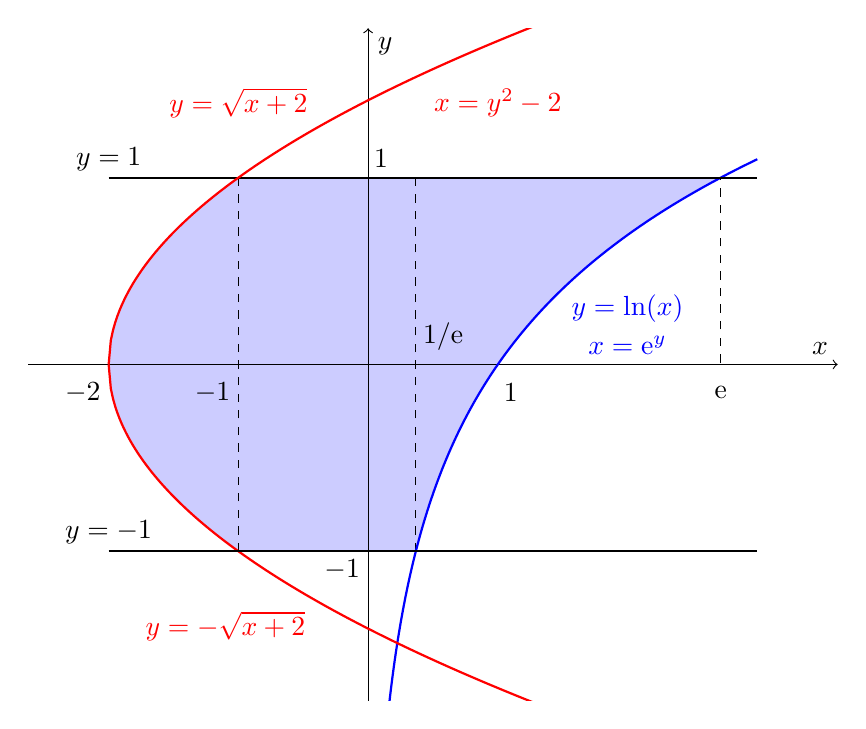
\begin{tikzpicture}
  \begin{axis}[
    scale=1.5,
    axis lines=center,
    xlabel={$x$},
    ylabel={$y$},
    xmin=-2.1, xmax=3.1,
    ymin=-1.5, ymax=1.5,
    samples=300,
    domain=-1:1,
    clip=true,
    ytick=\empty,
    xtick=\empty,
    enlargelimits=true,
    axis line style={->},
    xticklabel=\empty,
    yticklabel=\empty,
  ]

  \addplot [blue, thick, domain=1/e:1, draw=none, fill=blue!20] {ln(x)} \closedcycle;
  \addplot [blue, thick, domain=-1-0.01:1/e+0.01, draw=none, fill=blue!20] {-1} \closedcycle;
  \addplot [blue, thick, domain=-1-0.01:1+0.01, draw=none, fill=blue!20] {1} \closedcycle;
  \addplot [blue, thick, domain=-2:-1, draw=none, fill=blue!20] {sqrt(x+2)} \closedcycle;
  \addplot [blue, thick, domain=-2:-1, draw=none, fill=blue!20] {-sqrt(x+2)} \closedcycle;
  \addplot [blue, thick, domain=1:e, draw=none, fill=blue!20] {1} \closedcycle;
  \addplot [blue, thick, domain=1:e, draw=none, fill=white] {ln(x)} \closedcycle;
  
  \draw[black] (axis cs:0,-1) -- (axis cs:0,1);
  \draw[black] (axis cs:-2,0) -- (axis cs:e,0);
  \draw[white] (axis cs:e,0.01) -- (axis cs:e,1);
  \draw[dashed] (axis cs:-1,-1) -- (axis cs:-1,1);
  \draw[dashed] (axis cs:e,0.01) -- (axis cs:e,1);
  \draw[dashed] (axis cs:1/e,-1) -- (axis cs:1/e,1);

  \addplot [blue, thick, domain=0.1:3] {ln(x)};
  \addplot [thick, domain=-2:3] {1}; 
  \addplot [red, thick, domain=-2:3] {sqrt(x+2)};
  \addplot [red, thick, domain=-2:3] {-sqrt(x+2)};
  \addplot [thick, domain=-2:3] {-1};
  
  \node at (axis cs:e,-0.15) {$\mathrm e$};
  \node at (axis cs:1.1,-0.15) {$1$};
  \node at (axis cs:-2.2,-0.15) {$-2$};
  
  \node at (axis cs:0.1,1.1) {$1$};
  \node at (axis cs:-0.2,-1.1) {$-1$};
  
  \node at (axis cs:-1.2,-0.15) {$-1$};
  \node at (axis cs:1/e+0.21,0.15) {$1/\mathrm e$};
    
  \node[red] at (axis cs:1,1.4) {$x=y^2-2$};
  \node[red] at (axis cs:-1,1.4) {$y=\sqrt{x+2}$};
  \node[red] at (axis cs:-1.1,-1.4) {$y=-\sqrt{x+2}$};

  \node[blue] at (axis cs:2,0.3) {$y=\ln(x)$};
  \node[blue] at (axis cs:2,0.1) {$x=\mathrm e^y$};
  \node at (axis cs:-2,-0.9) {$y=-1$};
  \node at (axis cs:-2,1.1) {$y=1$};

  \end{axis}
\end{tikzpicture}\hspace{0.5cm}
\end{center}

\hfill

\noindent (i) The variable is $y$. Hence, the limits are $-1, 1$, respectively.

\[A=\int_{-1}^1\left[\mathrm{e}^y-(y^2-2)\right]\,dy\]

\hfill

\noindent (ii) We have three different regions. This leads us to take three different integrals.

\[A=\int_{-2}^{-1}\left[\sqrt{x+2}-(-\sqrt{x+2})\right]\,dx+\int_{-1}^{1/\mathrm{e}}\left[1-(-1)\right]\,dx+\int_{1/\mathrm{e}}^{\mathrm{e}}\left(1-\ln x\right)\,dx\]

\end{document}